\documentclass[11pt, oneside]{article} 
\usepackage{geometry}
\geometry{letterpaper} 
\usepackage{graphicx}
	
\usepackage{amssymb}
\usepackage{amsmath}
\usepackage{parskip}
\usepackage{color}
\usepackage{hyperref}

\graphicspath{{/Users/telliott_admin/Dropbox/Tex/png/}}
% \begin{center} 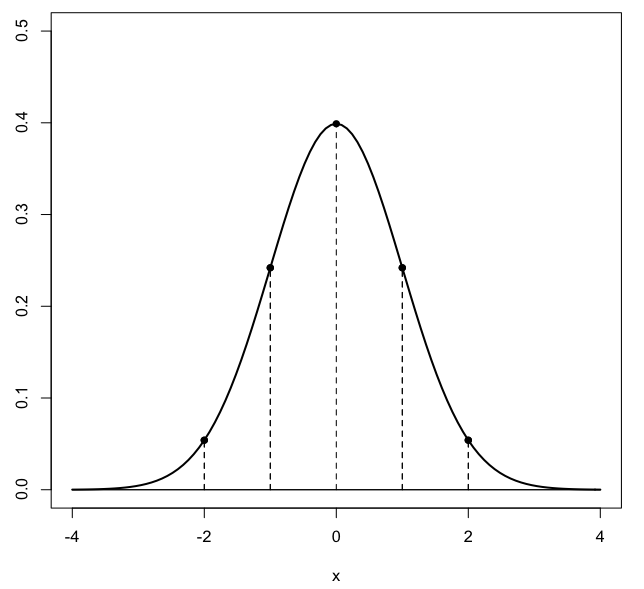
\includegraphics [scale=0.4] {gauss3.png} \end{center}

\title{Across the river (or not)}
\date{}

\begin{document}
\maketitle
\Large

The problem we want to solve is as follows.  There is a (very smooth) river that flows with a speed $u$, while you and your twin brother each swim with a speed $v$.  You have used your trigonometry skills to mark out a position which is up-river from the start point a distance equal to the width of the river, $d$.

Your brother wants to race (across and back versus up and down), and he's willing to let you pick which way you want to swim.  Which should you choose?

To solve this problem, first recall that the time to travel any distance $d$ at a constant speed $v$ is 

\[ t = d/v \]

Also, the time to swim up-river (and back) depends on your relative speed with respect to the land, going up-river it is $v-u$ and coming down-river it is $v+u$.  The total time for the first trip is

\[ t_1 = \frac{d}{v-u} + \frac{d}{v+u} = d(\frac{v + u + v - u}{v^2-u^2}) = \frac{2dv}{v^2-u^2}\]

For the second trip, across and back, you need to swim upstream at some angle $\theta$ in order that the current will sweep you back down to a point on the line that goes directly across the river.  The vectors make a little right triangle with hypotenuse $v$ and far side $u$.  The effective speed is $\sqrt{v^2 - u^2}$.  So, just as for the up and back trip, there is a requirement that $v > u$.  You should probably calculate $\theta$ before leaving shore, $\theta = \sin^{-1}(u/v)$.

Having calculated the speed, the time is just
\[ t_2 = \frac{2d}{\sqrt{v^2 - u^2}} \]

The ratio of the two times is

\[ \frac{t_1}{t_2} = \frac{2dv}{v^2-u^2} \frac{\sqrt{v^2 - u^2}}{2d} \]
\[ = \frac{v}{\sqrt{v^2 - u^2}} \]

Let's check this result quickly.  Suppose $v=5, u=3$ (in $m/s^2$).  Suppose we go up-river $7200 \ m$ at $2 \ m/s$ (taking 1 hr) and then back down-river $7200 \ m$ at $8 \ m/s$ for 0.25 hr or $5/4$ hr total.  

Pythagoras tells us that we go across the river at $4\  m/s$.  If the one-way distance is $7200 \ m$, then we do each half in $1800 s$ = 0.5 + 0.5 = 1.0 hr.  Going across is faster.

Which is a bit surprising.  The average speed up- and down-river is 5, yet we are slower than going across with a constant speed of 4.  That's because we already spent a whole hour at $2 \ m/s$ going up-river, we still have to come back!

There is a very famous experiment which depends on this difference.

\url{http://en.wikipedia.org/wiki/Michelson-Morley_experiment}

\end{document}  